\documentclass{article}
\usepackage[preprint]{neurips_2024}
\usepackage{amsmath,amssymb}
\usepackage{booktabs}
\usepackage{graphicx}
\usepackage{hyperref}
\usepackage{placeins}
\usepackage{tikz}
\usetikzlibrary{positioning,arrows.meta,calc,fit}

\newcommand{\vk}{\mathbf{k}}
\newcommand{\vv}{\mathbf{v}}
\newcommand{\vq}{\mathbf{q}}
\newcommand{\vx}{\mathbf{x}}
\newcommand{\vy}{\mathbf{y}}
\newcommand{\mW}{\mathbf{W}}


\title{Associative Memory Is the Model}

\author{
  jfg \\
  \texttt{fourierproject@gmail.com}
}

\begin{document}
\maketitle

\begin{abstract}
Transformers and state space models (e.g.\ Mamba) use sophisticated mechanisms to mix information across sequence positions. We argue that \textbf{associative memory does most of the work}, and the backbone needs only minimal local mixing. We augment language models with a Hebbian memory---a matrix of outer-product associations updated at each token---and systematically ablate the backbone. On The Stack (code), at 100M parameters: Mamba alone achieves 2.53 nats; adding Hebbian memory improves it to 1.82 nats; replacing Mamba's recurrence with a 4-token depthwise convolution gives 1.79 nats with no recurrence at all. At 124M parameters on FineWeb (natural language), Conv+Heb reaches 3.39 nats versus the nanoGPT 124M baseline of 3.28 nats---a small-scale gap that linear attention variants like RetNet close and surpass at larger scales. The sequence model backbone contributes only local feature extraction; \textbf{the associative memory handles nearly all long-range recall}.
\end{abstract}

\section{Introduction}

Transformers~\citep{vaswani2017attention} and state space models like Mamba~\citep{gu2024mamba,dao2024mamba2} use complex mechanisms---quadratic attention, selective gating, discretized recurrence---to capture long-range dependencies in sequences.

But what if associative memory, not the sequence model, is the primary mechanism for long-range reasoning? In this work, we decompose language modeling into two capabilities: first, \textbf{associative binding}---storing and retrieving associations across arbitrary distances---and second, \textbf{local feature extraction}---combining adjacent tokens into useful representations.

A Hebbian associative memory~\citep{hebb1949organization}---a decaying outer-product matrix updated at each token---handles the first almost entirely. For the second, a depthwise convolution over just 4 tokens suffices. The resulting architecture contains no recurrence, no attention, and no gating beyond SiLU, yet matches SSM-based models at comparable parameter counts and comes within 0.11 nats of nanoGPT on natural language.

Our key finding is stark: replacing Mamba with a 4-token convolution matches performance (1.79 vs 1.82 nats) at a fraction of the complexity, and a model with \emph{no} sequence mixing at all (pure linear projection + Hebbian) still converges to 3.18 nats. On FineWeb at 124M parameters, Conv+Heb reaches 3.39 nats versus the nanoGPT baseline of 3.28---a gap consistent with other linear attention variants at this scale, which close at larger scales~\citep{sun2023retentive}.

The associative memory is not merely an augmentation---it is nearly the entire model.

\section{Method}

\begin{figure}[t]
\centering
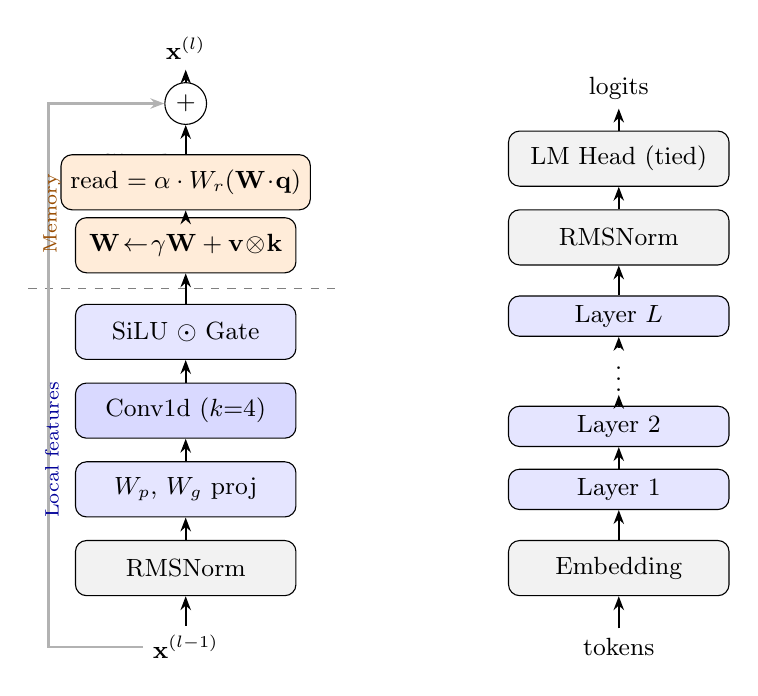
\begin{tikzpicture}[
    block/.style={draw, rounded corners, minimum width=2.8cm, minimum height=0.7cm, align=center, font=\small},
    op/.style={draw, circle, inner sep=2pt, font=\small},
    arr/.style={-{Stealth[length=5pt]}, thick},
    every node/.style={font=\small},
]
% === Single Layer (left) ===
\node[font=\normalsize\bfseries] at (0, 5.8) {Single Layer};

\node (in) at (0, -0.3) {$\vx^{(l-1)}$};
\node[block, fill=gray!10] (norm) at (0, 0.7) {RMSNorm};
\node[block, fill=blue!10] (proj) at (0, 1.7) {$W_p$, $W_g$ proj};
\node[block, fill=blue!15] (conv) at (0, 2.7) {Conv1d ($k{=}4$)};
\node[block, fill=blue!10] (gate) at (0, 3.7) {SiLU $\odot$ Gate};

% Divider
\draw[dashed, gray] (-2, 4.25) -- (2, 4.25);

\node[block, fill=orange!15] (write) at (0, 4.8) {$\mW \!\leftarrow\! \gamma\mW + \vv\!\otimes\!\vk$};
\node[block, fill=orange!15] (read) at (0, 5.6) {read $= \alpha \cdot W_r(\mW \!\cdot\! \vq)$};

\node[op] (add) at (0, 6.6) {$+$};
\node (out) at (0, 7.3) {$\vx^{(l)}$};

\draw[arr] (in) -- (norm);
\draw[arr] (norm) -- (proj);
\draw[arr] (proj) -- (conv);
\draw[arr] (conv) -- (gate);
\draw[arr] (gate) -- (write);
\draw[arr] (write) -- (read);
\draw[arr] (read) -- (add);
\draw[arr] (add) -- (out);

% Residual
\draw[arr, gray!60] (in.west) -- ++(-1.2,0) |- (add.west);

% Labels
\node[font=\scriptsize, blue!60!black, rotate=90] at (-1.7, 2.2) {Local features};
\node[font=\scriptsize, orange!60!black, rotate=90] at (-1.7, 5.2) {Memory};

% === Full Stack (right) ===
\node[font=\normalsize\bfseries] at (5.5, 5.8) {Full Model};

\node (emb_in) at (5.5, -0.3) {tokens};
\node[block, fill=gray!10] (emb) at (5.5, 0.7) {Embedding};

\node[block, fill=blue!10, minimum height=0.5cm] (l1) at (5.5, 1.7) {Layer 1};
\node[block, fill=blue!10, minimum height=0.5cm] (l2) at (5.5, 2.5) {Layer 2};
\node at (5.5, 3.2) {$\vdots$};
\node[block, fill=blue!10, minimum height=0.5cm] (lL) at (5.5, 3.9) {Layer $L$};

\node[block, fill=gray!10] (fnorm) at (5.5, 4.9) {RMSNorm};
\node[block, fill=gray!10] (head) at (5.5, 5.9) {LM Head (tied)};
\node (logits) at (5.5, 6.8) {logits};

\draw[arr] (emb_in) -- (emb);
\draw[arr] (emb) -- (l1);
\draw[arr] (l1) -- (l2);
\draw[arr] (l2) -- ++(0, 0.4);
\draw[arr] (5.5, 3.5) -- (lL);
\draw[arr] (lL) -- (fnorm);
\draw[arr] (fnorm) -- (head);
\draw[arr] (head) -- (logits);

\end{tikzpicture}
\caption{Architecture overview. \textbf{Left}: A single layer. The conv block (blue) extracts local features over 4 tokens. The Hebbian memory (orange) writes and reads associative bindings via a $D{\times}D$ outer-product matrix. \textbf{Right}: The full model stacks $L$ identical layers with tied embeddings.}
\label{fig:arch}
\end{figure}

The model (Figure~\ref{fig:arch}) stacks $L$ identical layers with pre-norm residual connections:
\begin{equation}
    \vx^{(l)} = \vx^{(l-1)} + \text{HebbianMemory}(\text{Conv}(\text{RMSNorm}(\vx^{(l-1)})))
\end{equation}
Each layer contains a local feature extractor (depthwise convolution) and a Hebbian associative memory. Token embeddings are tied with the output projection.

\paragraph{Parameter count} For our 100M model ($L{=}12$, $D{=}1024$, $E{=}2$, $d_\text{conv}{=}4$), per layer:
\begin{itemize}
    \item Conv block: $3ED^2 + ED \cdot d_\text{conv} \approx 6.3\text{M}$ (projections + conv kernel)
    \item Hebbian memory: $2D^2 + 2 \approx 2.1\text{M}$ (write/read projections + decay/alpha)
    \item Total per layer: $\sim$8.4M; 12 layers: $\sim$100M
\end{itemize}

\FloatBarrier

\subsection{Hebbian Associative Memory}

At each position $t$, the model maintains a memory matrix $\mW_t \in \mathbb{R}^{D \times D}$ that accumulates outer-product associations between consecutive representations:
\begin{align}
    \mW_t &= \gamma \mW_{t-1} + \vv_t \otimes \vk_{t-1} \label{eq:write} \\
    \text{read}_t &= \mW_{t-1} \cdot \vq_t \label{eq:read}
\end{align}
where $\vv_t = W_v \vx_t$ is the value projection, $\vk_t = \vx_t$ is the write key (the raw hidden state), $\vq_t = \vx_t$ is the read query, and $\gamma = \sigma(\delta)$ is a learned decay with $\delta$ initialized to 4.6 ($\gamma \approx 0.99$). Here $\vx_t$ denotes the output of the conv block at position $t$. The layer output combines the conv output with the memory read:
\begin{equation}
    \vy_t = \vx_t + \alpha \cdot W_r \cdot \text{read}_t
\end{equation}
where $\alpha = \exp(\log \alpha_0)$ is a learned per-layer memory strength (initialized at 0.03) and $W_r$ is a learned read projection. A residual connection from the layer input is added on top. Both $\alpha$ and $\gamma$ are learned per layer.

For training, we use a chunkwise parallel form with chunk size $C$, running in $O(TC \cdot D + T \cdot D^2)$ time; at inference, the recurrent form (Equations~\ref{eq:write}--\ref{eq:read}) runs in $O(D^2)$ per step.

\subsection{Convolution Backbone}

Each layer's local feature extractor is a gated depthwise convolution:
\begin{align}
    \vx' &= \text{SiLU}(\text{Conv1d}(W_p \vx)) \odot \text{SiLU}(W_g \vx) \\
    \text{out} &= W_o \vx'
\end{align}
where $W_p, W_g \in \mathbb{R}^{D \times ED}$ project to an expanded dimension ($E{=}2$), Conv1d is a causal depthwise convolution with kernel size $d_\text{conv}{=}4$, and $W_o \in \mathbb{R}^{ED \times D}$ projects back. This block sees exactly $d_\text{conv}$ tokens of local context. All long-range information flows through the Hebbian memory.


\section{Experiments}

All models are $\sim$100M parameters ($d_\text{model}{=}1024$), trained on The Stack for 4000 steps with sequence length 2048, batch size 1 (no gradient accumulation), cosine schedule with peak $3 \times 10^{-4}$ and 500-step warmup. Layer counts vary to match parameter budgets (11--15 layers; see Table~\ref{tab:backbone}). We report average validation loss over steps 2000--4000 in nats (natural log cross-entropy). Validation is noisy at batch size 1, so we average across eval points.

\subsection{Backbone Ablation}

Our central experiment replaces the backbone while keeping the Hebbian memory identical. Both use learned decay $\gamma$ (init 0.99); Mamba+Heb uses a fixed $\alpha{=}0.04$, Conv+Heb uses learned per-layer $\alpha$ (init 0.03). Table~\ref{tab:backbone} shows results.

\begin{table}[h]
\caption{Backbone ablation on The Stack ($\sim$100M params, 4000 steps).}
\label{tab:backbone}
\centering
\begin{tabular}{lccc}
\toprule
\textbf{Model} & \textbf{Layers} & \textbf{Params} & \textbf{Avg Val Loss} \\
\midrule
Conv(4) + Heb & 12 & 102.9M & 1.79 \\
Mamba + Heb & 11 & 98.5M & 1.82 \\
Mamba (no Heb) & 15 & 102.1M & 2.53 \\
\bottomrule
\end{tabular}
\end{table}

\textbf{Hebbian is the dominant mechanism.} Removing Hebbian memory from Mamba degrades performance from 1.82 to 2.53 nats ($+$0.71). The memory contributes far more than the backbone.

\textbf{Conv matches Mamba with no recurrence.} Conv+Heb achieves 1.79 nats, slightly better than Mamba+Heb at 1.82 nats. The convolution has no SSM recurrent state yet matches a full state space model.

\begin{figure}[h]
\centering
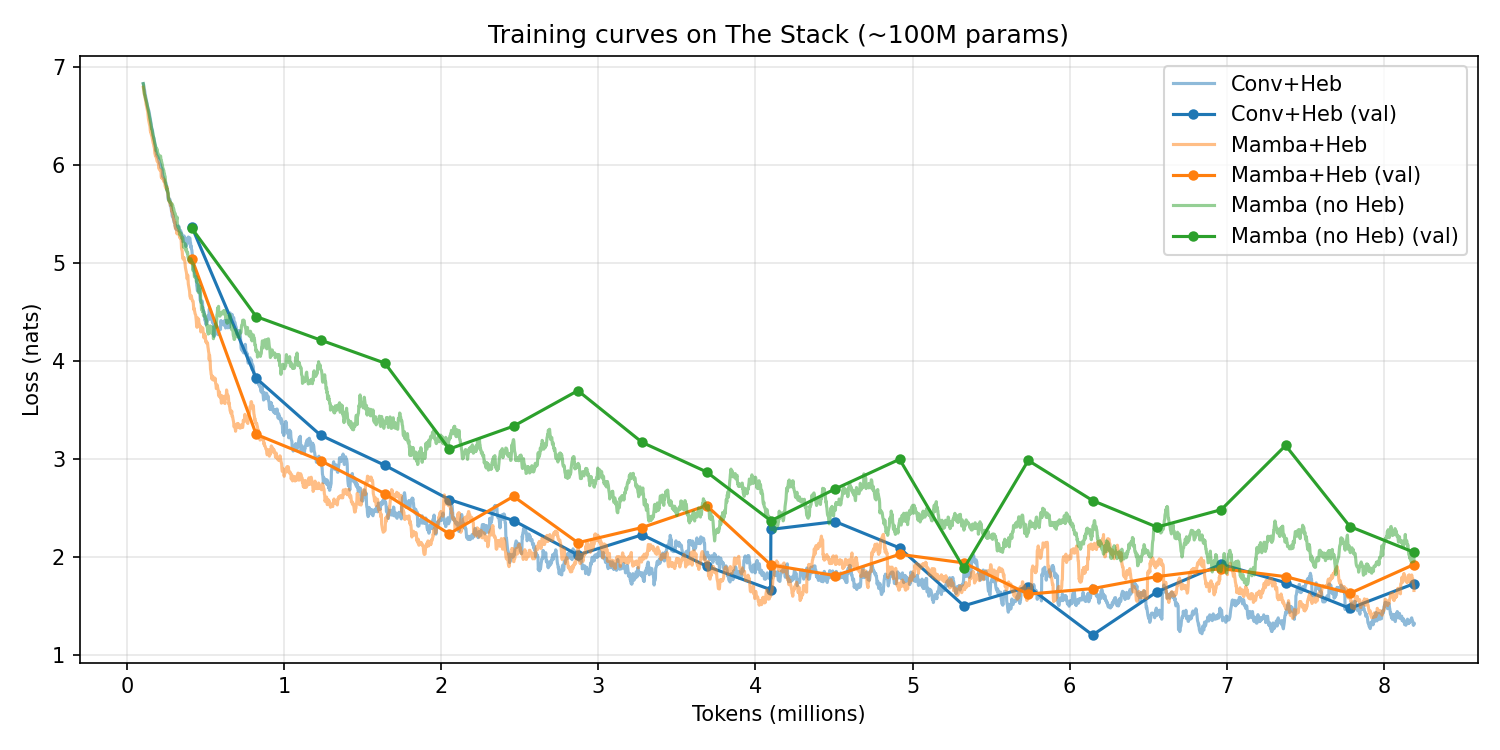
\includegraphics[width=\textwidth]{figures/val_loss_comparison.png}
\caption{Training curves on The Stack ($\sim$100M params, $\sim$8M tokens). Solid lines show smoothed training loss; markers show validation loss. Conv+Heb tracks Mamba+Heb throughout training, while Mamba without Hebbian memory lags by $\sim$0.7 nats.}
\label{fig:training}
\end{figure}

\subsection{Recurrent Inference}

We evaluate all three models using their recurrent (autoregressive) form on 4096-token windows from The Stack validation set, averaging over 8 windows. Table~\ref{tab:recurrent} shows per-segment losses.

\begin{table}[h]
\caption{Recurrent inference on The Stack (4096 tokens, 8 windows). Loss in nats by position segment.}
\label{tab:recurrent}
\centering
\begin{tabular}{lcccc|c}
\toprule
\textbf{Model} & \textbf{0--1K} & \textbf{1--2K} & \textbf{2--3K} & \textbf{3--4K} & \textbf{Overall} \\
\midrule
Mamba (no Heb) & 1.98 & 1.87 & 2.05 & 1.99 & 1.97 \\
Conv+Heb & 1.46 & 1.35 & 1.47 & 1.44 & 1.43 \\
Mamba+Heb & 1.30 & 1.40 & 1.51 & 1.25 & \textbf{1.37} \\
\bottomrule
\end{tabular}
\end{table}

Both memory-augmented models outperform Mamba alone by 0.5+ nats, confirming that the Hebbian memory drives the improvement. Mamba+Heb edges out Conv+Heb by 0.06 nats in recurrent mode---Mamba's recurrence provides a small benefit for autoregressive generation over long contexts, though the gap is minor compared to the 0.60-nat contribution of the memory itself. All models show stable loss across sequence length.

\subsection{Learned Memory Parameters}

The Conv+Heb model learns per-layer memory strength $\alpha$ and decay $\gamma$. Figure~\ref{fig:learned} shows the learned values after 4000 steps.

\begin{figure}[h]
\centering
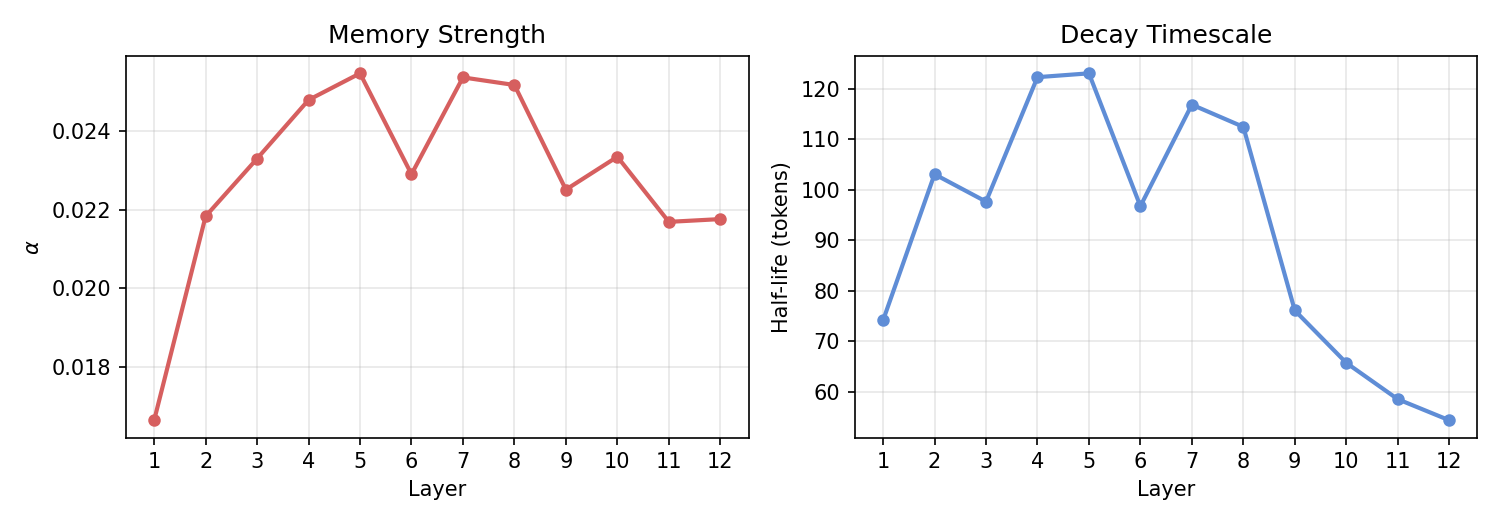
\includegraphics[width=\textwidth]{figures/learned_params.png}
\caption{Learned per-layer parameters in the 100M Conv+Heb model. \textbf{Left}: Memory strength $\alpha$ peaks in middle layers ($\sim$0.025) and drops at boundaries ($\sim$0.017). \textbf{Right}: Decay half-life ($\log 2 / \log(1/\gamma)$) shows a timescale hierarchy---early layers retain memory longer ($\sim$120 tokens), later layers decay faster ($\sim$55 tokens).}
\label{fig:learned}
\end{figure}

The $\alpha$ profile suggests middle layers perform the bulk of associative reasoning, while boundary layers focus on local features (early) and decoding (late). The decay hierarchy means early layers build broad context while later layers focus on recent associations.

\subsection{FineWeb Scaling}

To test generalization beyond code, we train a 124M-parameter Conv+Heb model on FineWeb~\citep{penedo2024fineweb}, a large-scale English web corpus, and compare against the nanoGPT 124M transformer baseline (3.28 nats).

\paragraph{Baseline} The target is 3.28 nats, the validation loss achieved by Karpathy's nanoGPT 124M reproduction in llm.c~\citep{karpathy2024llmc}---a GPT-2-architecture transformer (12 layers, $D{=}768$, 12 heads) trained with AdamW on $\sim$10B tokens of FineWeb with GPT-2 tokenization (vocab 50,304) and sequence length 1024.

\paragraph{Our setup} Conv+Heb uses 18 layers, $D{=}768$, expand factor 2, $d_\text{conv}{=}4$, with learned per-layer $\alpha$ (init 0.03) and $\gamma$ (init 0.99). Training uses AdamW ($\beta_1{=}0.9$, $\beta_2{=}0.95$), cosine schedule with peak $\text{lr}{=}6 \times 10^{-4}$ decaying to $6 \times 10^{-5}$, 500-step warmup, weight decay 0.1, gradient clipping at 1.0, and bf16 autocast. We train for 19,000 steps with 524K tokens per step ($\sim$10B tokens total), matching the baseline's token budget. Training was done on a single H100 GPU with \texttt{torch.compile}.

\begin{figure}[h]
\centering
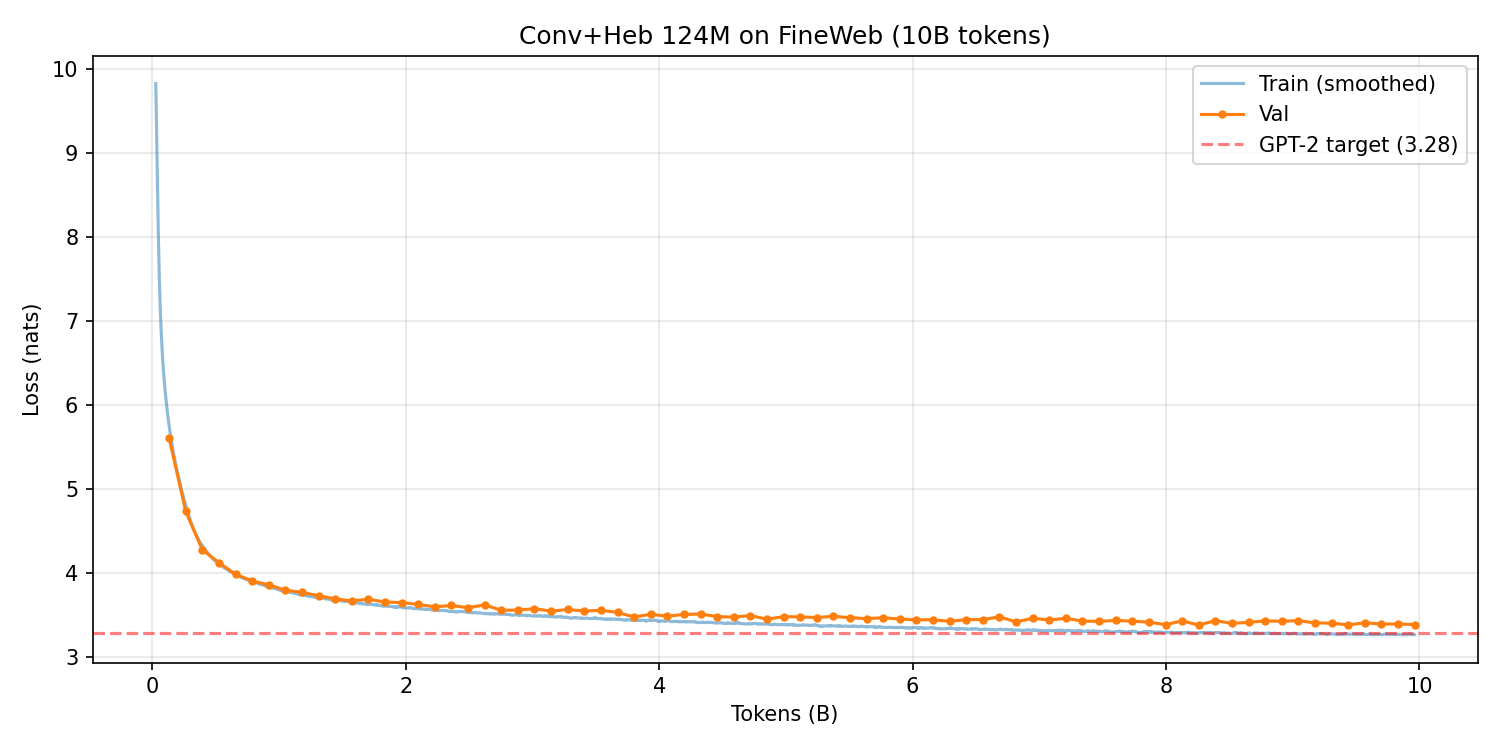
\includegraphics[width=\textwidth]{figures/fineweb_curve.png}
\caption{Conv+Heb (124M params) on FineWeb. The dashed line shows the nanoGPT 124M baseline (3.28 nats). Final validation loss: 3.39 nats, a gap of 0.11 nats.}
\label{fig:fineweb}
\end{figure}

Conv+Heb reaches 3.39 nats versus the baseline of 3.28 nats---a gap of 0.11 nats. Both models use AdamW with comparable training recipes and the same token budget. The 0.11-nat difference is consistent with the small-scale behavior of linear attention variants (RetNet, GLA, DeltaNet), which show similar gaps at 124M--350M parameters but close and even surpass transformers at larger scales---RetNet at 6.7B achieves lower perplexity than its transformer baseline~\citep{sun2023retentive}. The gap likely reflects scale, not a fundamental limitation of the memory mechanism.

\section{Discussion}

\paragraph{Hebbian memory as the dominant mechanism}
The $+$0.71 nat gap between Mamba and Mamba+Heb versus the 0.03-nat gap between Mamba+Heb and Conv+Heb points to a clear decomposition: the memory is doing the work. The outer-product matrix is content-addressable---retrieval is by similarity to the query, not by temporal position---making it fundamentally different from SSM recurrence, which compresses history into a fixed-size state vector.

This echoes complementary learning systems in neuroscience~\citep{mcclelland1995complementary}: neocortex for slow feature learning, hippocampus for fast associative binding. The Hebbian memory plays the hippocampal role.

\paragraph{Connection to fast weight programmers and linear attention}
Our memory is an instance of fast weight programming~\citep{schmidhuber1992learning,ba2016using,schlag2021linear}. Linear attention~\citep{katharopoulos2020transformers} maintains the same outer-product matrix without decay; adding learnable decay connects to RetNet~\citep{sun2023retentive} and GLA~\citep{yang2024gated}. Our contribution is not the mechanism itself, but the finding that \emph{it alone, paired with a trivial backbone, suffices for competitive language modeling}.

\paragraph{Limitations}
Our 100M-parameter models are trained on only $\sim$8M tokens (The Stack), which is significantly undertrained by modern standards. The FineWeb experiment uses a full 10B-token budget but is limited to 124M parameters. Scaling to larger models and longer training would strengthen the comparison.

\section{Related Work}

\paragraph{State space models}
S4~\citep{gu2022efficiently} introduced structured state spaces for sequence modeling. Mamba~\citep{gu2024mamba} added input-dependent selection, achieving strong performance on language modeling. Mamba-2/SSD~\citep{dao2024mamba2} revealed the duality between SSMs and structured attention, enabling efficient multi-head implementations. Our work shows that for models augmented with associative memory, the SSM backbone can be replaced with a simpler alternative.

\paragraph{Associative memory and fast weights}
Our Hebbian memory follows the fast weight lineage~\citep{schmidhuber1992learning,ba2016using,schlag2021linear} and is closely related to linear attention~\citep{katharopoulos2020transformers}, RetNet~\citep{sun2023retentive}, GLA~\citep{yang2024gated}, and RWKV~\citep{peng2023rwkv}. Hopfield networks~\citep{hopfield1982neural,ramsauer2021hopfield} provide an energy-based alternative. Our contribution is showing that these mechanisms make the surrounding architecture largely redundant.

\section{Conclusion}

A 4-token depthwise convolution paired with Hebbian outer-product memory matches a 100M-parameter Mamba+Heb on code language modeling---with no recurrence. Removing the memory costs 0.71 nats. Replacing the SSM with a trivial convolution costs 0.03 nats in parallel training and 0.06 nats in autoregressive inference. On FineWeb at 124M parameters, Conv+Heb reaches within 0.11 nats of nanoGPT 124M---a gap consistent with other linear attention variants that closes at larger scales.

The backbone is not irrelevant---the 0.11-nat gap on FineWeb shows it contributes something, likely precise short-range token interactions. But it is not the dominant mechanism. The bulk of language modeling performance comes from associative storage, and the complexity of modern SSMs and attention is disproportionate to their contribution. Future work should focus on the memory, not the backbone.

\bibliography{references}
\bibliographystyle{plainnat}

\end{document}
